\documentclass[11pt, a4paper]{article}

% Packages
\usepackage[utf8]{inputenc}
\usepackage[T1]{fontenc}
\usepackage{geometry}
\geometry{a4paper, margin=1in}
\usepackage{graphicx}
\usepackage{amsmath, amssymb, amsfonts}
\usepackage{booktabs} % For professional tables
\usepackage{hyperref}
\usepackage{float}
\usepackage{caption}
\usepackage{subcaption}
\usepackage{xcolor}
\usepackage{listings}
\usepackage{tikz} % Added for drawing the graph
\usepackage[style=ieee, backend=biber]{biblatex}

% Bibliography source
\addbibresource{references.bib}

% Title Information
\title{\textbf{Low-Bit Quantized nanoGPT Speedrun: Testing the Effects of Weight and Activation Quantization}}

\author{
    \textbf{Travis Hammond} \\
    \textit{Whiting School of Engineering} \\
    \textit{Johns Hopkins University} \\
    Baltimore, USA \\
    \texttt{thammo19@jhu.edu}
}
\date{\today}

\begin{document}

\maketitle

\begin{abstract}
The scaling of Large Language Models (LLMs) is increasingly bottlenecked by memory bandwidth and energy consumption. The emerging 1.58-bit (ternary) quantization paradigm offers a potential solution by constraining weights to $\{-1, 0, 1\}$, thereby enabling matrix multiplication to be approximated by integer addition. This research implements and evaluates a low-bit quantized GPT architecture from scratch, based on the \texttt{modded-nanogpt} codebase. We conduct a comparative study on the FineWeb-10B dataset to isolate the impact of quantizing different model components. Specifically, we examine three configurations: (1) Ternary Weights only ($W_{1.58}A_{BF16}$), (2) Ternary Weights with Quantized Attention ($W_{1.58}A_{QK}$), and (3) Fully Quantized Weights and Activations ($W_{1.58}A_{1.58}$). Our results demonstrate that weight-only ternary quantization provides a strong balance between performance and efficiency, achieving a validation loss of 3.41 (comparable to the 3.28 baseline). Conversely, we find that aggressive quantization of activations to ternary values without specific architectural adaptation leads to significant performance degradation (Loss 3.87).
\end{abstract}

\section{Introduction}
As Large Language Models (LLMs) grow in size, the computational cost of training and inference has become a critical barrier to deployment. Traditional 16-bit (BF16/FP16) operations dominate memory traffic, creating a "memory wall" where compute units idle while waiting for data. Quantization-Aware Training (QAT) addresses this by simulating low-precision arithmetic during the training phase, allowing the network to adapt to discretization noise.

Recent foundational work, such as BitNet b1.58 \cite{ma2024era}, suggests that extreme quantization to ternary values $\{-1, 0, 1\}$ is feasible. This "1.58-bit" representation allows for the replacement of heavy floating-point Multi-Accumulate (MAC) operations with lighter integer addition and subtraction.

In this work, we investigate the practical trade-offs of this paradigm by implementing a quantized GPT-2 model from scratch via a speedrun training regime. Our primary objective is to decouple the effects of weight quantization from activation quantization. We hypothesize that while full quantization offers maximum theoretical speedups, \textbf{weight-only ternary quantization} provides the majority of memory benefits with significantly higher training stability.

\section{Background}

\subsection{1.58-bit Quantization}
The 1.58-bit scheme constrains parameters to three possible states: $\{-1, 0, 1\}$. This reduces the memory requirement per parameter to $\log_2(3) \approx 1.58$ bits.
\begin{itemize}
    \item \textbf{Memory Efficiency:} Storing weights in ternary format drastically reduces the model footprint compared to FP16 or INT8.
    \item \textbf{Computational Efficiency:} Matrix multiplication $Y = XW$ becomes a sparse addition process.
\end{itemize}

\subsection{Smooth Gradient Approximation}
Training discrete variables prohibits standard backpropagation because the rounding function has a derivative of zero almost everywhere. While the Straight-Through Estimator (STE) is a common solution, it often leads to gradient mismatch. Instead, we adopt a smooth gradient approximation for the backward pass \cite{semenov2025smooth}.  This method approximates the gradient of the rounding operation using a differentiable power function centered at the transition points, providing a more informative signal to the latent high-precision weights during optimization.

\section{Methods}

\subsection{Implementation}
We modified the optimized \texttt{modded-nanogpt} repository to support custom quantization. We distinguish between the \texttt{Quantize} layer (applied to weights) and specific activation quantization functions (applied to inputs and features).

\subsubsection{Weight Quantization ($W_{1.58}$)}
We utilize an absolute-mean quantization strategy. For a weight matrix $W$, we compute a scaling factor $\gamma = \text{mean}(|W|)$. The weights are scaled and rounded:
\begin{equation}
    \tilde{W} = \text{Round}\left(\frac{W}{\gamma}\right) \times \gamma
\end{equation}
Crucially, while the forward pass uses a standard round, the backward pass utilizes a custom smooth approximation. For an input $x$ and smoothness parameter $k=5$, the gradient is computed as:
\begin{equation}
    \frac{\partial \tilde{W}}{\partial W} \approx \text{clamp}\left(\frac{1}{k} \left| x - \text{round}(x - 0.5) - 0.5 \right|^{\frac{1}{k}-1}, -3, 3\right)
\end{equation}
Unlike approximations that peak at the decision boundary to force transitions, this function exhibits a local minimum at the boundary (0.5, 1.5). The gradient magnitude increases as the value approaches the integer targets, aggressively penalizing deviations from the discrete states $\{-1, 0, 1\}$ once the weight is "captured" by a bin, while still maintaining a non-zero gradient at the boundary to allow for state switching.

\subsubsection{Activation Quantization and Architecture}
We apply specific quantization functions to activations depending on the target bit-width. For 8-bit targets (such as inputs to Linear layers), we use a symmetric \textbf{Linear} quantization. For 1.58-bit targets, we utilize \textbf{Tanh} or \textbf{Sigmoid} functions to constrain values before rounding.

The modified data flow for the Multi-Head Attention (MHA) and MLP blocks is as follows:

\noindent \textbf{Attention Block:}
\begin{align*}
    X_{in} &\leftarrow \text{PreQuant}(X) \quad \text{(Linear 8-bit or Tanh 1.58-bit)} \\
    Q, K, V &\leftarrow \text{Linear}(X_{in}, \text{Quant}(W_{QKV})) \\
    Q, K &\leftarrow \text{ActQuant}(Q), \text{ActQuant}(K) \quad \text{(Linear 8-bit or Tanh 1.58-bit)} \\
    Y &\leftarrow \text{FlashAttn}(Q, K, V) \\
    Y_{out} &\leftarrow \text{Linear}(Y, \text{Quant}(W_{out}))
\end{align*}

\noindent \textbf{MLP Block:}
\begin{align*}
    X_{in} &\leftarrow \text{PreQuant}(X) \\
    H &\leftarrow \text{Linear}(X_{in}, \text{Quant}(W_{fc})) \\
    H_{act} &\leftarrow \text{ActQuant}(H) \quad \text{(ReLU}^2 \text{ 8-bit or Tanh 1.58-bit)} \\
    Y_{out} &\leftarrow \text{Linear}(H_{act}, \text{Quant}(W_{proj}))
\end{align*}

\subsection{Experimental Setup}
\begin{itemize}
    \item \textbf{Architecture:} We utilize the \texttt{modded-nanogpt} architecture, a modernized GPT-2 implementation featuring significant kernel optimizations and architectural improvements for high-efficiency training.
    \item \textbf{Hardware:} Training was conducted on a single NVIDIA H100 GPU. \textit{Note: The Extreme Full Quant run utilized an H100 SXM variant, while other experiments used standard PCIe H100s.}
    \item \textbf{Dataset:} FineWeb-10B (Tokenized).
    \item \textbf{Optimization:} We employ the specialized optimization regime native to the \texttt{modded-nanogpt} codebase, trained for a total of \textbf{2,285 steps}.
\end{itemize}

\section{Experiments and Results}

We conducted four distinct experiments to isolate the impact of quantizing specific model components.

\subsection{Experimental Configurations}
\begin{enumerate}
    \item \textbf{Baseline:} Standard BF16 precision for all weights and activations.
    \item \textbf{Weights Only ($W_{1.58}$):} Weights constrained to $\{-1, 0, 1\}$. Activations remain BF16.
    \item \textbf{Weights + Attn Act ($W_{1.58}A_{QK}$):} Weights are ternary. Attention Q/K activations are quantized to 8-bit/ternary.
    \item \textbf{Extreme Full Quant ($W_{1.58}A_{1.58}$):} Both weights and activations (MLP and Attn) are aggressively quantized to low-bit representations.
\end{enumerate}

\subsection{Quantitative Analysis}
Table \ref{tab:results} presents the final validation loss and training speed for each configuration.

\begin{table}[H]
\centering
\caption{Comparison of Validation Loss and Training Speed on FineWeb-10B}
\label{tab:results}
\setlength{\tabcolsep}{12pt} % Increases column spacing for better readability
\begin{tabular}{@{}lcccc@{}}
\toprule
\textbf{Experiment} & \textbf{Config} & \textbf{Val Loss} & \textbf{Step Time (ms)} \\ \midrule
1. Baseline & BF16 & \textbf{3.2773} & 706.65 \\
2. Weights Only & $W_{1.58} / A_{BF16}$ & 3.4105 & 726.32 \\
3. Weights + QK & $W_{1.58} / A_{QK}$ & 3.4894 & 751.22 \\
4. Extreme Full & $W_{1.58} / A_{1.58}$ & 3.8690 & \textbf{556.06*} \\ \bottomrule
\end{tabular}
\vspace{0.2cm} % Spacing between table and note
\begin{minipage}{0.9\linewidth}
    \footnotesize \textit{*Note: The Extreme Full run was conducted on an H100 SXM, contributing to the lower step time alongside bandwidth savings.}
\end{minipage}
\end{table}

\subsubsection{Weight Quantization Performance}
The \textbf{Weights Only} model (Exp 2) demonstrated high resilience. Despite reducing the information capacity of the weights to 1.58 bits per parameter, the validation loss increased by only $\approx 0.13$ compared to the BF16 baseline.

\subsubsection{Collapse in Extreme Quantization}
The \textbf{Extreme Full Quantization} (Exp 4) suffered a severe cost to model quality (Loss 3.87). While the step time was significantly lower (556ms), this is partially attributed to the use of superior hardware (H100 SXM) for this specific run. However, the loss degradation suggests that aggressive discretization of activations destroys necessary semantic information in the attention and MLP bottlenecks.

\subsection{Ablation on Activation Functions}
We conducted micro-ablations (400 steps) to select optimal activation functions for the low-bit regimes.
\begin{itemize}
    \item \textbf{Tanh Activations:} Val Loss 4.40
    \item \textbf{Sigmoid Activations:} Val Loss 4.85
\end{itemize}
The superior performance of Tanh suggests that zero-centered distributions are easier to map to ternary states $\{-1, 0, 1\}$ than positive-only Sigmoid distributions. Consequently, we utilized Tanh for 1.58-bit activation paths and Linear quantization for 8-bit paths.

\begin{figure}[H]
    \centering
    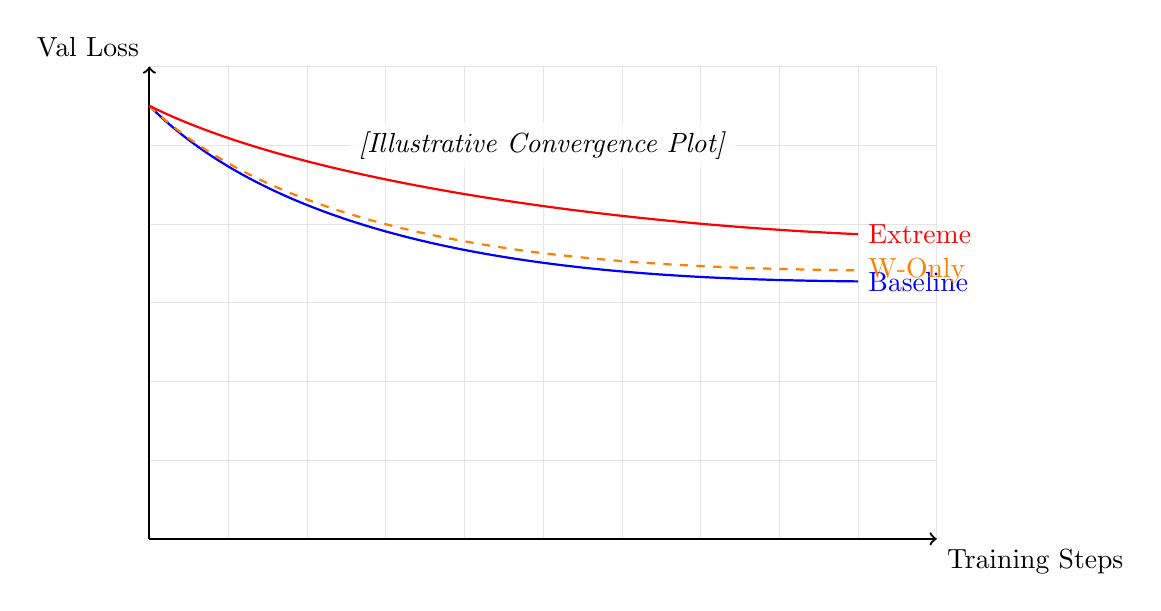
\begin{tikzpicture}
        % Draw grid
        \draw[step=1cm,gray!20,very thin] (0,0) grid (10,6);
        
        % Draw axes
        \draw[thick,->] (0,0) -- (10,0) node[anchor=north west] {Training Steps};
        \draw[thick,->] (0,0) -- (0,6) node[anchor=south east] {Val Loss};
        
        % Illustrative curves
        % Baseline (Blue) - lowest loss
        \draw[blue, thick] (0,5.5) .. controls (2,3.5) and (6,3.3) .. (9,3.27) node[right] {Baseline};
        
        % Weights Only (Orange/Dashed) - slightly higher
        \draw[orange, dashed, thick] (0,5.5) .. controls (2,3.6) and (6,3.45) .. (9,3.41) node[right] {W-Only};
        
        % Extreme (Red) - plateaus high
        \draw[red, thick] (0,5.5) .. controls (2,4.5) and (6,4.0) .. (9,3.87) node[right] {Extreme};
        
        % Label for plot area
        \node[align=center, fill=white, opacity=0.8, text opacity=1] at (5,5) {\textit{[Illustrative Convergence Plot]}};
        
    \end{tikzpicture}
    \caption{Convergence comparison. The Weight-Only ternary model (Orange) tracks the BF16 Baseline (Blue) closely, while the Extreme Quantization model (Red) plateaus at a significantly higher loss.}
    \label{fig:convergence}
\end{figure}

\section{Conclusion}
This study confirms the viability of 1.58-bit weight quantization for Large Language Models trained from scratch. Our findings highlight a crucial distinction:
\begin{enumerate}
    \item \textbf{Weights are robust:} Constraining weights to $\{-1, 0, 1\}$ using smooth gradient approximation works effectively, yielding acceptable loss with reduced memory footprint.
    \item \textbf{Activations are sensitive:} Simple ternary quantization of activations (via Tanh or Sigmoid) leads to performance collapse. 8-bit linear quantization remains a safer alternative for activation paths.
\end{enumerate}

\section{Impact and Future Work}
These results facilitate the deployment of LLMs on memory-constrained consumer hardware. Future work should investigate:
\begin{itemize}
    \item \textbf{Scaling Laws:} Verifying if the performance gap between W1.58 and BF16 diminishes at larger parameter scales (e.g., 7B+), as predicted by BitNet literature \cite{wang2023bitnet}.
    \item \textbf{Advanced Activation Quantization:} Exploring learnable activation clipping or more sophisticated smooth approximations to stabilize fully quantized training.
\end{itemize}

\printbibliography

\end{document}
